\documentclass[11pt,twoside,bibtotoc]{scrartcl}
%\documentclass[12pt, a4paper]{article}

\newif\ifpdf
\ifx\pdfoutput\undefined
\pdffalse % we are not running PDFLaTeX
\else
\pdfoutput=1 % we are running PDFLaTeX
\pdftrue
\fi

\ifpdf
\usepackage[pdftex]{graphicx}
\else
\usepackage{graphicx}
\fi

\usepackage{ucs}
\usepackage[utf8x]{inputenc}
%\usepackage[T1]{fontenc}
\usepackage[english]{babel}
%\usepackage{german}
%\usepackage{longtable}
%\usepackage{tocbibind}
%\usepackage{makeidx}
\usepackage[pdftex,pageanchor,colorlinks,pdfborder=0,breaklinks,urlcolor=blue]{hyperref}
\usepackage{amsmath}
\usepackage{amsfonts}
\usepackage{amssymb}
\usepackage{units}
%\usepackage{pdfsync}  % enable tex source and pdf output syncronicity
%\usepackage[all]{xy}
\usepackage{multicol}
%\usepackage{rotating}
%\usepackage{wrapfig}
%\usepackage{subfigure}
%\usepackage{listings}

\usepackage{geometry} % to change the page dimensions
\geometry{a4paper}
\geometry{textwidth=16.0cm,textheight=24.5cm}
\geometry{left=3.0cm,twoside}
\parskip=0 cm
\parindent=0.0cm

\renewcommand{\baselinestretch}{1.2}

\newcommand{\mytitle}{Tool support for user testing of stereoscopic fatigue}

\usepackage{fancyhdr} % This should be set AFTER setting up the page geometry
\pagestyle{fancy} % options: empty , plain , fancy
\fancyfoot{}
\fancyfoot[LE,RO]{\textrm{\thepage}}
\fancyfoot[LO,RE]{\textit{Roethlin, G. 2008}}

\renewcommand{\labelitemi}{-}

\newcommand{\todo}[1]{{\LARGE TODO: #1}}

% Depth of the TOC
%\setcounter{secnumdepth}{3}
%\setcounter{tocdepth}{2}

\hypersetup{
    pdftitle={\mytitle},
%    pdfsubject={Subject of the document}, % Subject 
    pdfauthor={Gerhard Roethlin},              % Author
    pdfkeywords={master, fatigue testing software, stereo vision},       % Keywords
}

\title{Master Thesis: \mytitle\\
{\large Designing and implementing a flexible and extensible testing framework}}
\author{\normalsize Gerhard R\"othlin 
{\texttt{\href{mailto:cbreak@the-color-black.net}{cbreak@the-color-black.net}}}}
\date{2008.01.07 - 2008.07.07}

\ifpdf
\DeclareGraphicsExtensions{.pdf, .jpg, .tif}
\else
\DeclareGraphicsExtensions{.eps, .jpg}
\fi

\begin{document}

\maketitle

\begin{center}
\includegraphics[width=15cm,clip,trim=0cm 0cm 0cm 0cm]{media/title.png}
\end{center}

\begin{multicols}{2}

\begin{abstract}
Viewing stereoscopic movies or images is unnatural. The focus and vergence of the eyes have to be decoupled. Artefacts and inconsistencies of a stereoscopic image with the real world cause confusion and decrease viewing pleasure.

Topic of this thesis is to write a Tool that enables exploration of those problems and quantifying them by providing a flexible and extensible framework for user testing. Challenges include understanding the needs in this relatively new field of research, as well as the commonly used methods in user testing.
\end{abstract}

\section{Introduction\label{Introduction}}
\paragraph{}
Researching the effect of the viewing of stereoscopic stimuli requires a different tool than usual user testing.
While traditional tests only require simple input and often don't need to react on it, changing the stimuli based on what happened is often a requirement for the tests planned in stereoscopic vision research.
The stimuli have to be more complex than simple bitmap images as those in standard user tests.

Which features would simplify the creation and conduction of such tests?
How can a tool be flexible enough to support every imaginable type of test, while still be user friendly?
What is the right tradeoff between power and usability?

The following sections will introduce several examples of use cases, tests in which the framework should enhance the procedures and lessen the work done in test design and execution.
In the features section, some important abilities needed in those tests are detailed.


\subsection{Program Design}
\paragraph{}
\todo{Give overview over program design part}

\subsection{Implementation}
\paragraph{}
\todo{Give overview over implementation part}

\subsection{Documentation}
\paragraph{}
\todo{Give overview over documentation part}


%\part{Design}
\section{Design\label{Design}}
\paragraph{}
Implementing a flexible and powerful framework for user testing of stereoscopic problems requires a design that accounts for some special requirements. To find out what those requirements are, several tests where designed and executed. The design of the application was adapted to be fit for use in those and many other imaginable tests.

\paragraph{Creation}
The framework is split into three parts: The test design part aids with the construction of the test scene. A scene is a description of stimuli, possible inputs, and reactions to them. Traditional tests in this area show a series of pictures, requiring user feedback for each, while measuring the response time and the correctness. Stimuli are often precomputed and only consist of a single pixel image.

The requirements for stereoscopic test are different: It is not feasible to manually prepare stimuli, especially if complexe interaction is required. A method to generate them on the fly is needed.
Section \ref{sceneRep} describes how the look of a scene could be represented.

\paragraph{Testing}
The testing part is the most important. It displays stimuli and logs the user replies, reacting in a way that is defined by the designer of the test. While traditional tests only follow the question-response pattern, stereoscopic user tests often require more: Trials often have to be randomized with several constraints, simply randomizing might lead to overlaps, or imbalances in dependent properties. All parameters of the stimulus have to be directly or indirectly controllable based on user input such as movement of stimuli, movement of the camera, or visibility of objects.

\paragraph{Analysis}
Analysing the gathered data is the third part. This is usually done in a combinataion of \textit{Microsoft Excel} and highly specialized data analysation methods such as Anova. Both are sophisticated and well known by the users.

The easiest way to achieve compatibility with the known procedures is to produce data in a format, that is evaluatable in those tools. A log transformation program can take care of this in most tests: The time stamp based logs get parsed, and challenge-response times get measured and written in a format importable by spread sheet applications.
For more flexible data access, it can be imported into a database, where standard \textit{SQL} queries can be used to select subsets of the data, sorted and filtered in many ways.

Some tests might not follow this pattern, and the data has to be analysed in a different way.


\subsection{Representation of a Scene\label{sceneRep}}
\paragraph{}
\textit{Scene graphs} are used to store scenes in a structured way. They have been continually developed since their invention\cite{scenegraph} to account for spatial, state, hierarchy and other properties.
Many scene graph libraries exist, but they are usually focused on a specific field, and part of a bigger framework.

To be able to control inconsistencies such as individual depth cues, it is required that the scene graph can represent these. Nodes could add or remove cues for their children, giving a maximum of control to the users. Scene graph libraries do not support those requirements. Designing a simple scene graph is required.

\subsubsection{Node types}
\paragraph{}
Scene graphs are tree structures consisting of nodes with zero or more child nodes. The scene itself is typically the root node, while actual rendered objects often are leaves. The following nodes are planed to be implemented in the framework.

\begin{description}
\item[Rectangle] A primitive geometry node, which has the shape of a parallelogram. The node can reference a texture, which gets mapped on it's surface.
\item[Parallelepiped] A primitive geometry node, which has the shape of a parallelepiped (parallelogram prism). As it's parent it can be textured.
\item[Pixelplane] A primitive geometry node. It is used to draw pixel exact images at any position in space. It requires a texture to be visible. Pixelplanes are point shaped, and therefore are not influenced by scaling and rotation.
\item[Text] A primitive geometry node. It draws text at any position in space, similar to Pixelplanes.
\item[Mesh] A primitive geometry node who's geometry is defined by a mesh. The mesh can contain vertex normals and vertex texture coordinates. A texture can be mapped on the object. It might be desirable to also include vertex color.
\item[AffineTransformation] A group  node. It contains other nodes, which it can affine transform by directly manipulating the matrix stack.
\item[Camera] A group node. It contains other nodes, which are rendered by this camera instead of the global camera. This is used to control projection cues in a consistent way. Has to reset the depth buffer.
\item[DepthBuffer] A group node. Disables or enables the use of the depth buffer for all contained elements. This is used to disable occlusion clues. Can reset the depth buffer.
\item[Lighting] A group node. Enables lighting and a light source with controllable parameters for all sub nodes. This is used to enable lighting depth cues.
\item[Atmosphere] A group node. Enables the fog equation and controls its parameters. This is used to enable aerial depth cues.
\end{description}

\paragraph{}
The following nodes are problematic and might be hard to use, implement and understand due to their side effects.

\begin{description}
\item[XSize] A group node that scales objects to add or remove depth cues caused by perspective projection. It can be implemented on object (scale object individually, without consider intra object depth) or space level (scale  as function of depth, which is similar to a camera projection). Either way has it's own problems.
\item[XOffsest] A group node that moves objects it contains as function of their camera distance. Can be used to add or remove height-of-field, convergence or motion parallax cues.
\end{description}

\subsubsection{Node organisation}
\paragraph{}
Nodes are the building blocks of a scene graph, but how they are put together is similarly important. Due to the requirements of some nodes to clear the depth buffer, and the DepthBuffer node, the order of objects in a group node has to be in the desired order of drawing, not insertion.

Since most advanced functionality is designed to be in group nodes, objects have to be grouped based on their semantics. Those are drawn perspectively in the same camera node, all that have the be lit in a lighting node, and so on. For some nodes this is required for them to work, for others it is just a matter of performance.

To increase performance in complex scenes it might be desirable to use a spatially organized tree. Instead of grouping by state (such as camera, lighting), grouping would be done by proximity. This allows for faster culling. To get both functionalities, parallel trees have to be built. An object would reside in both trees. But so far, scene complexity is intended to be very low, so this optimisation is unlikely to be needed.


\subsection{Mechanics of a Scene\label{sceneMech}}
\paragraph{}
Having a scene with the desired visualisation is not enough. To conduct a test, the scene has to react to user input, to timers and has to be able to modify the scene graph. Logging has to be unconstrained. Randomisation and random permutations require a state.

\subsubsection{``Programming'' a scene}
\paragraph{}
The solution to all those problems is to use a programming language to define the scene mechanics. Anything that can be computed is assumed to be computable with a language that is \textit{turing complete}\cite{turing}. Using such a language would not limit the possibilities of the user, while making designing the scene much easier, faster and less error prone than writing a dedicated tool.

\subsubsection{Procedual API}
\paragraph{}
\textit{Procedural languages} are turing complete, so embedding a language would give all the computational flexibility needed. The same methods to build a scene graph and change object properties within \textit{C++} code can also be used in the scene mechanics. Proxy objects can mediate between the embedded language and the \textit{C++} API.

Creating scenes this way follows standard programming paradigmas, and someone who can program in a procedural language should have little problems adapting to what ever syntax the embedded language uses. The drawback of this approach is, that someone who does not have programming experience will find creating a scene rather unintuitive.

\subsubsection{State API}
\paragraph{}
A more user friendly approach is \textit{Visual Programming}, a class of languages that are based on a visual instead of a textual representation of programs. Visual languages are used in data acquisition tools such as \textit{National Instruments}' \textit{LabVIEW}, music studio software such as \textit{Cycling '74}'s \textit{Max/MSP} or scripting tools like \textit{Apple}'s \textit{Automator}.
The pattern used in those languages is that of \textit{Dataflow-Programming}\cite{dataflow}. Unfortunately, it does not fit into the requirements of the testing tool.

Popular graphic languages in education are \textit{Finite State Machines}\cite{fsm}. They are easy to describe mathematically, and are rather intuitive, compared to traditional programming languages.
The original \textit{LEGO} \textit{Mindstorms} used a flow chart based language that is loosely related with Finite State Machines, and managed to appeal even to young people without programming experience.

A finite state machine is an algorithm that is described as set of states, and state transitions. The transitions can follow various rules, but the most common are based on input. A transition can also write output, or do various other things, depending on the type of state machine.

The original turing machine is a finite state machine that can also write on a so called ``tape''.


\section{Cues\label{Cues}}
\paragraph{}
Seeing stereo is not only based on binocular stereopsis.There are several aspects of the visual impression that allow the perception of depth. Common depth cues include accommodation, aerial perspective, binocular disparity, convergence, height in visual field, motion perspective, occlusion, relative size, and relative density. In addition others have been suggested, such as linear perspective, light and shading and texture gradients.%, kinetic depth, kinetic occlusion and disocclusion, and gravity.

Cutting and Vishton\cite{DepthCues} analyzed nine of these depth cues to asses their relative strength. Those cues will be described in the following paragraphs, and their reproduction or elimination on screen in a digitally generated scene is discussed. The use of \textit{OpenGL} or a similar technology is assumed, techniques like ray-tracing or vector based painting may require different methods. A summary can be found in table \ref{DepthCuesTable}.


\subsection{Projection based cues}
\paragraph{}
These cues are caused by the way the 3D world gets projected onto the 2D surface of the retina.
Even though the reason that each of them exists is the same, the way they are evaluated and their reproduction is different.

Most projections\cite{proj} that are in use, map a ray in the world space onto a single point in the image space. \textit{Parallel Projection}\cite{parallel} and \textit{Perspective Projection}\cite{perspective} are the most commonly used methods. Real optics use a projection similar to perspective projection.

Since all the following cues are generated by the same cause, enabling and disabling each is not possible in a consistent way. There are two basic ways to get partial individual control despite this: Compensate  the perspective projection of the camera by removing cues, or  adding cues to a parallel projection. Careless use of either method can cause conflicts such as pinning, rivalry, or the inability to fuse the image.
Using two cameras might require depth ordering, since the depth buffer has to be invalidated.


\subsubsection{Relative size}
\paragraph{Description}
The size of objects relative to each other is a strong clue for their distance, but it requires knowledge or assumptions about the size of an object. Due to the \textit{perspective projection}, objects further away from a viewer take up less space in it's field-of-view. When seeing a human, it's distance can be estimated fairly accurately.

Seeing an unknown object requires comparisons with other objects in the scene. Upon seeing a number of cubes with different perceived sizes, and without prior knowledge of their size, one could assume similarity in size, and derive depth relations between them.

\paragraph{Reproduction}
Relative size only works when the perceived size of an object changes with it's distance. Using a perspective camera is an easy way to do this. When creating an artificial image, the size change can also be simulated by non-uniformly scaling objects based on their distance to the camera. If the whole object is considered as a single entity, artefacts might occur. In the case of OpenGL or most RayTracers, both parallel and perspective cameras are available.

\paragraph{Non-reproduction}
If the size of objects is not intended to change with their distance from the viewer, either choosing a parallel projection or compensating the projection based scaling by scaling the object size is needed. This causes visual distortions, if the object is embedded in a scene that is subject to relative size.


\subsubsection{Relative density}
\paragraph{Description}
Relative density is closely related to relative size. It concerns the projected density of objects, which are distributed regularly. When such a group of objects change in depth, or take up different depth areas, their change in perceived density yield information about the depth change.

\paragraph{Reproduction}
If a perspective projection is used, relative density changes are calculated correctly. Introducing relative density clues into a scene that is rendered with a parallel projection requires non uniform scaling.

\paragraph{Non-reproduction}
Eliminating the relative depth cue from part of a scene that is parallel projected requires non uniform scaling of a group of objects. Both the position relative to each other, and the size relative to each other of the objects has to change.


\subsubsection{Motion perspective}
\paragraph{Description}
Motion perspective is closely related with relative size and relative density. When moving and looking sideways, objects seem to move into the opposing direction. Objects that are far move much slower than objects that are close. When passing objects, their relative ordering can even change: A mountain that was on the right side of a tree can be seen on it's left side. This is caused by the projection into image space, which makes the space far away appear smaller, and therefore objects moving in this space slower.

\paragraph{Reproduction}
As with the other projection based clues it appears naturally if a perspective projection is used. Without this, it can still be reproduced by moving objects at a velocity scaled with the distance to the camera.

\paragraph{Non-reproduction}
Compensating motion perspective in a perspective scene requires the scaling of the embedded space, or the movement speed relative to the camera. This can lead to inconsistencies with other parts of the image.


\subsubsection{Height in visual field}
\paragraph{Description}
The bottom parts of objects that are touching the ground can be seen at the same place in the retina as the part of the floor they rest on. This is caused by the projection from the world into image space. The assumption are that the objects are touching the ground, that the ground is reasonably even, and that the viewer is perpendicular and above to the floor plane.

\paragraph{Reproduction}
Reproducing changes of objects in the height in visual field is fairly straight forward. The effect can be achieved by use of a projection that fulfills this property, such as a perspective projection, or some parallel projections. Or by simply translating objects in image space. Care has to be taken to not cause visual artefacts such as pinning.

\paragraph{Non-reproduction}
Eliminating the effect of the projection on the height in the visual field is straight forward. A projection that maps the floor plane on one single line in image space also maps the bottom of all objects on that plane. Objects can be shifted in image space to compensate for the projection. Raising objects so that they float above the ground is unproblematic, but moving them below ground either leads to occlusion, or depth conflicts.


\subsubsection{Convergence}
\paragraph{Description}
When moving a camera in a plane, the camera has to rotate to keep an object in the center of the image. The same is the case when using two cameras, or two eyes. Keeping a real object in focus will lead to converging eyes, since they have to point inwards, or for objects at infinitely long distance have to be parallel. The amount of convergence allows judging the distance. This is similar to the method of triangulation\cite{triangulation} used in navigation. Since the eye distance of humans is about 65mm, only close objects can be judged reliable.

Convergence \textit{(Proprioception)}is very closely related to height-of-fiel, motion parallax and binocular stereopsis, since it is created by the same effect. The way humans perceive it is very different.

\paragraph{Reproduction}
Reproducing convergence clues requires the creation of separate images for each eye. It comes natural with perspective projections and two cameras. Alternatively, the shift of paralaxe can also be simulated just by shifting the object horizontally depending on it's distance of the camera.

\paragraph{Non-reproduction}
Not reproducing convergence clues either requires to not use a perspective (or converged) projection, or to compensate the movement in paralaxe by moving the object horizontally in the scene depending on the camera distance.


\subsubsection{Binocular disparity and stereopsis}
\paragraph{Description}
Binocular stereopsis is similar to convergence, but it is based on the perception of the same object from two viewpoints, and analyising the differences. To be effective, the cameras have to be at different positions relative to each other. Adult human eyes are separated by about 65mm. Perceiving from different points of view is also closely related with motion perspective, and the same strategies can be applied to it.

\paragraph{Reproduction}
Reproducing binocular disparities that can be fused for binocular stereopsis is easy with two parallel cameras with perspective projection, or converged cameras with parallel/perspective projection.
Achieving the same effect by horizontally shifting object positions is possible, but suffers from several drawbacks. Objects will appear to be flat \textit{(cardboarding)}. Shifting objects horizontally is also used to create other stereo cues, so they will clash.

\paragraph{Non-reproduction}
Removing binocular stereopsis in a scene is fairly simple, reducing the camera separation to zero achieves it with little side effects.


\subsection{Other cues}
\paragraph{}
The following cues are not dependent on each other, or the projection of the scene, and can therefore be easier enable and disabled individually.

\subsubsection{Occlusion}
\paragraph{Description}
Objects that are in front of other objects relative to the viewer are perceived to occlude the object behind. Even transparent or translucent objects often change the appearance of objects they occlude. This allows to infer depth ordering of objects. This clue is very strong, and it's range is the longest of all depth cues. It does however not allow to judge the distance between objects.

\paragraph{Reproduction}
Reproducing this depth clue digitally requires extra work, since most output media do not have a notion of depth. A traditional approach is the Painter's Algorithm\cite{painters}. Objects are ordered by depth and drawn from far to close. Ordering objects has performance implications, and is not always possible.
A newer method that does not require sorting is the Depth Buffer\cite{zbuffer} (also known as Z-Buffer). For every pixel it's associated depth value is stored. New objects only replace pixels further away.

\paragraph{Non-reproduction}
Not reproducing this clue is fairly straight forward. Disabling the depth buffer allows ordering objects according to preferred depth appearance, independently of their actual depth coordinates. Objects that are both behind and in front of an other object have to be segmented into pieces. This is most commonly the case when objects intersect.

Objects that consist of several surfaces might require internal ordering to appear correct, which is expensive. One way to resolve this problem is to clear the depth buffer after every object drawing. Depending on the size of the image this might be costly also.


\subsubsection{Aerial perspective}
\paragraph{Description}
Areal perspective is related with Occlusion: Objects far away from the viewer are often occluded by the atmosphere, be it air, smoke, fog or water. Consequentially, objects far away change their appeared color, losing saturation, and chroma.
Unlike most depth cues, it gets more effective as the distance from the observer increases.

\paragraph{Reproduction}
Reproducing this cue requires extra work. A common approach is to mix the object color with a fog color, depending on it's distance to the observer. This is cheap, and can be enabled per object\cite{fog}. Weights of the mixing is determined by a fog equation.

\paragraph{Non-reproduction}
Not reproducing this clue is easy, and it is not enabled by default. Explicit control over the appeared depth can be achieved by individually changing the fog equation for each object.


\subsubsection{Accomodation}
\paragraph{Description}
Accommodation is the change in the shape of the lens of the eye, to keep the perceived image of the world sharp\cite{accommodation}. It is coupled with convergence. Viewing stereoscopic material requires that the accommodation stays the same, since all image information comes from a screen at a fixed depth.

\paragraph{Reproduction}
Artificially generating the requirement that the human eye changes accommodation is hard. It requires optics in between the eye and the screen, or the changing of distance to screen depending on the object that is focused. Neither is practical to do interactive.

\paragraph{Non-reproduction}
Not reproducing this cue is almost required. Everything seen on a screen requires the same accommodation to be viewed as the screen itself. If a constant accommodation requirement throughout the scene exists, a screen at a huge distance, or a convex screen can be used.


\subsubsection{Light and Shading}
\paragraph{Description}
Shading and lighting is a strong cue for depth inside of objects. Shadows, or varying light intensities based on the angle to the light source all fall in this category.
Shadows are created by objects obstructing the light from falling onto an object. The shape depends on the position and shape of the obstructing object, the target, and the light source. Creating shadows is a hard problem in real time computer graphics.
Shading an object is coloring it based on the amount of light that falls on it's surface. This depends on the type, distance and shape of the light source, and the angle of incident on the surface, and is easily approximated even in real time computer graphics.

\paragraph{Reproduction}
Shading can be enabled and disabled per object, or even per vertex.
Shadows require more work, and it depends on the algorithm used for creating them how easy it is to add one to a scene.
Creating shadows on planar surfaces are easier than shadows on arbitrary shapes.

\paragraph{Non-reproduction}
Removing a shadow is hard, but not creating one is easy, so this is the recommended course of action.

\begin{table*}[p]
\begin{center}
\small
\begin{tabular}{p{2cm}|p{1.9cm}|p{5cm}|p{5cm}}
Cue & Family & Created by & Removed by \\
\hline
Relative Size &
Projection &
Perspective Projection or non uniform scaling as a function of distance to camera &
Parallel projection or non uniform scaling as a function of distance to camera \\
Relative Density &
Projection &
Perspective Projection or non uniform scaling of space and objects, or translation and scaling of objects as a function of distance to camera &
Parallel Projection or non uniform scaling of space and objects, or translation and scaling of objects as a function of distance to camera \\
Motion Perspective &
Projection &
Perspective Projection, scaling of space, or adjusting velocity of objects as function of camera distance &
Parallel Projection, scaling of space, or adjusting velocity of objects as function of camera distance \\
Height of visual field &
Projection &
Perspective Projection, an angled projection, angled camera, translating/shearing as function of distance to camera &
Parallel projection with camera parallel to ground plane, vertical translation/shearing as function of camera distance \\
Convergence &
Projection &
Two cameras with separation, either converged, perspective, or both. Or horizontal translation/shearing as function of distance to camera and camera direction &
Only one camera, parallel projection, horizontal translation/shearing as function of distance to camera and camera direction \\
Binocular stereopsis &
Projection &
Two cameras with separation, either converged, perspective, or both. Or horizontal translation/shearing as function of distance to camera and camera direction &
Only one camera, parallel projection, horizontal translation/shearing as function of distance to camera and camera direction \\
Occlusion &
Physical &
Depth ordering, Depth buffering &
Depth ordering, Blending \\
Aerial perspective &
Physical &
Fog Equation &
Not using Fog Equation \\
Accom\-modation &
Optical &
Adaptive optics, placing objects/screen at varying distances from viewer &
Default behaviour, whole screen requires at approximately the same accommodation \\
Light \& Shading &
Physical &
Light Equation, Shadow projection, shadow maps &
Not using Light Equation, Shadow projection or shadow maps
\end{tabular}
\end{center}
\caption{List of cues with a short summary on how to create and remove them}
\label{DepthCuesTable}
\end{table*}

%\part{Implementation}
\section{Implementation\label{Implementation}}
\paragraph{}
This section presents selected implementation details, describes the technologies in detail, and the tradeoffs that where taken.

\subsection{Used Frameworks\label{frameworks}}
\paragraph{}
When developing an application, it is impossible to write everything from scratch.
Frameworks and libraries help developers not spending time on reinventing wheels,
but on finding solutions to the specific problems of their program.

\ER\ uses several libraries for window management, memory management, scripting and rendering.


\subsubsection{Qt\label{FrameworkQt}}
\paragraph{}
A big part of the functionality comes from the operating system and associated platform APIs.
This includes basic necessities like reading data from a file, drawing data to screen or specialized functionality like drawing a tree view, scaling images or managing tool windows.

\paragraph{}
All operating systems offer their own API to do some of those things.
\textit{POSIX} is supported on Linux, Mac OS X and Windows, but it only covers basic file IO, and nothing graphical.
Specific APIs like \textit{Mac OS X'}s \textit{Cocoa} or Windows' \textit{.Net} have a much richer feature set, but limit the application to that platform.
This might be acceptable for widely distributed end user applications where a fraction of potential users can be ignored,
but in a research environment the software has to be able to use existing hardware optimally.
A solution is \textit{Qt}\cite{qt}:

\begin{quotation}
Qt is a cross-platform application framework for desktop and embedded development. It includes an intuitive API and a rich C++ class library, integrated tools for GUI development and internationalization, and support for Java™ and C++ development.
\end{quotation}

\paragraph{}
An alternative would be to use \textit{Java} with it's associated APIs, but it's support for hardware accelerated drawing is lacking.


\subsubsection{Boost\label{FrameworkBoost}}
\paragraph{}
\textit{C++} is an old language, and has it's root in the language \textit{C}.
Neither has advanced memory management tools, be it a garbage collector like \textit{LUA} or \textit{Java}, or a reference counting system like used in \textit{Objective-C}.
Managing memory manually is a challenge, doing it wrong can cause crashes that are hard to debug.

A solution to this problem is offered by \textit{TR1}, an extension to the C++ standard library.
Boost\cite{boost} is a provider of a \textit{TR1} implementation.

\paragraph{}
\textit{TR1} contains among others a robust and flexible implementation of a set of shared-ownership smart pointers.
As long as a smart pointer to a memory location exists, it can be used like a normal pointer thanks to \textit{C++}'s operator overloading,
but as soon as all pointers to it go out of scope, the memory will be automatically deallocated.

\paragraph{}
An other useful feature in boost are function binders.
while standard \textit{C} functions and static functions can be pointed at by a simple pointer,
\textit{C++} class member functions require more data
(Method Pointers vary in size depending on compiler and platform, and can be 12 bytes or more).
Together with the strict type checking of \textit{C++}, this makes storing pointers to member functions complicated and inflexible.

With \textit{TR1}'s functional library, binding any kind of method or function and storing it is easily possible, while still retaining strict type checking.
This is used to implement callbacks.


\subsubsection{OpenGL\label{FrameworkOpenGL}}
\paragraph{}
Since the whole goal of the tool is to generate stereoscopic stimuli and present them to test subjects,
the graphical rendering framework is of tremendous importance.
In the beginning of graphical computers, programs drew everything on their own, and accessed the frame buffer directly.
In modern systems, drawing is highly abstracted and often hardware accelerated.

\ER\ requires the ability to draw 3D scenes and reproduce many effects such as lighting, cameras, atmospheric effects and other depth cues.
The goal is to be able to test both abstract scenes consisting only of few shapes and a limited amount of cues,
as well as scenes that contain many cues, and more closely approximate real visuals.
This is similar to what computer games use.

\paragraph{}
The only cross platform 3D drawing toolkit is \textit{OpenGL}\cite{opengl}, a standard developed by \textit{Silicon Graphics} in 1992.
It's a state-driven procedural C API that was extended with many additions to the standard since it's inception.
Many features of \textit{OpenGL} are accelerated by modern graphic cards, and allow real time animation rendering.

The \ER\ renderer uses \textit{OpenGL} for the scene output.
Objects paint them-selfs with OpenGL commands.
The offerings of the framework are not perfect, but it allowed to realize almost all desired features.
A more advanced anaglyph renderer would likely be possible to do with frame buffer objects and pixel shader, but that would exclude a wide range of older installations and hardware.


\subsubsection{LUA\label{FrameworkLua}}
\paragraph{}
It was clear from the beginning of the project that the only way to get the required flexibility to do anything, and test anything can not be achieved by simply defining a scene format and some animation paths.
Tests like a flight simulator for motion sickness require interactivity in complex ways.
The chosen solution was to use a programming language to specify interaction and mechanics of a test.
The design of a language is complex, and many scripting languages are already established, so it was decided to reuse an existing language.

Most scripting languages are either intended to be used in stand-alone scripts such as \textit{Perl} or various shell scripting languages.
\textit{Python} can be used as  embedded language, and offers a very rich API on it's own.
The downside is that it is huge and comes with many features that are not needed, which complicate
the integration into custom applications.

\paragraph{}
The chosen language is \textit{LUA}\cite{lua}, a small library designed to be used as embedded language.
It provides all basic features, comes with garbage collection, flexible syntax and powerful binding API.
It's syntax is easy to understand, but still offers enough sugar to use not only procedural, but also modular, object oriented or functional programming.
It's license is very liberal, which made it popular even in the comercial game industry.
The official project description emphasizes those points.

\begin{quotation}
Lua is an extension programming language designed to support general procedural programming with data description facilities. It also offers good support for object-oriented programming, functional programming, and data-driven programming. Lua is intended to be used as a powerful, light-weight scripting language for any program that needs one. Lua is implemented as a library, written in clean C (that is, in the common subset of ANSI C and C++).
\end{quotation}

\paragraph{LuaBridge}
While the \textit{LUA} C API is very powerful, it is also very low level.
Writing code that interacts with \textit{LUA} and especially code that is called by it requires following the calling convention of \textit{LUA}.
Manually handling the low level API helped with understanding the language better and finding problems,
but it also required to maintain two interfaces, one that exposes functions to \textit{C++} and a second set for \textit{LUA}.

\textit{LuaBridge} automatically generates this binding code in a very elegant way.
Unlike tools like \textit{tolua++} it does not require a preprocessor,
it uses template meta programming to generate wrapper code.
\textit{LuaBind} works similar, but \textit{LuaBridge} is smaller, easier to understand and has less dependencies.




\subsection{Program}
\paragraph{}
The class \lstinline{Program} encapsulates a test scene.
It contains the scene graph (see \ref{SceneGraph}) and the scene mechanics (see \ref{Mechanic}).

The program mediates user input and relays it to the engine
and handles loading and storing of a scene.

The scene also manages names.
Names are important especially for serialisation, since lua variables are referred to by name.
Uniqueness and validity is ensured, and reserved lua keywords are protected.

\paragraph{Internal interaction}
In the current implementation, the scene mechanic code accesses the scene graph directly,
and has references to the actual objects.
This makes modularisation more difficult, and makes it impossible to replace a whole scene graph with a duplicate.
An improvement would be to only refer to objects by name or with some sort of \textit{URI}.
Implementing such a scheme would require a huge effort especially due to the nature of the binding to \textit{lua}.
\textit{LuaBridge} does not support polymorphism.




\subsection{Scene Graph}

%\begin{figure*}[htb]
\begin{center}
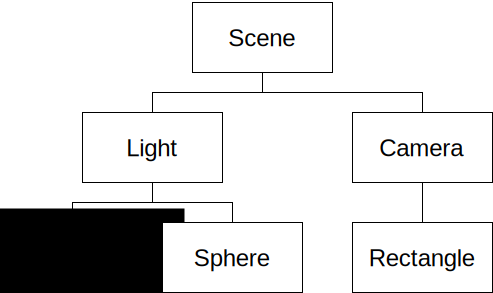
\includegraphics[width=7cm]{media/scene.pdf}
%\caption{A diagram of a possible scene graph.\label{imgScene}}
\end{center}
%\end{figure*}

\paragraph{}
The scene graph is organized by state.
State modifying containers contain visual objects.
The scene is a special container.

\subsubsection{Objects}
Most objects represent a visual shape.
They are organized in an inheritance hierarchy, all based on the class \texttt{Object}.
This hierarchy heavily relies on polymorphism, so there are several virtual member functions that can be customized.

An object offers visibility through drawing itself in OpenGL and persistence by writing itself to lua code.
An objects can also return a smart pointer to itself.
Clone creates an exact deep copy of the object.
For the UI, it can return a dialog that directly changes the parameters of the object.
Other classes can install handlers into an object to be notified when it is modified.

For more details please refer to the header file (see page \pageref{object.h}) or the doxygen documentation.
For an overview of objects, see section \ref{nodeTypes}.

\subsubsection{Special nodes\label{RendSpecial}}
\paragraph{}
\todo{Write about special nodes that have not been mentioned before}

\paragraph{Depth Buffer}
\paragraph{Light}
\paragraph{Fog}


\subsubsection{Surfaces}




\subsection{Mechanic}
\paragraph{}
\todo{Write about scene mechanics}
\todo{Write about lua}



\subsection{Rendering}
\paragraph{}
Rendering the scene into a perceivable image is one of the core jobs of the application.
Realizing effects that approximate both real movie footage and the wishes of the user is often hard, or even impossible.
The implementation is closely tied to the abilities requested from the tool, many effects such as lighting or arbitrary depth ordering requires low level trickery with the chosen framework.

In addition, the scene does not only have to be rendered once but often twice.
Binocular vision infers depth relationships from slight differences in images taken from two separate viewpoints.

Section \ref{FrameworkOpenGL} discusses the choice of drawing framework.
Section \ref{RendCamera} discusses how a 3D scene gets mapped into a 2D image.
Section \ref{RendStereo} discusses stereo rendering methods.
Section \ref{RendSpecial} discusses the implementation of other effects.
For a high level description of many features see section \ref{sceneRep} on scene representation and \ref{Cues} on the topic of depth cues.


\subsubsection{Camera\label{RendCamera}}
\paragraph{}
\todo{Write about why it is important, in OpenGL}
\todo{Write about parallel perspective, parallel converged}

\subsubsection{Stereo\label{RendStereo}}
\paragraph{}
Ideally, the output of the program is either intended to be viewed without binocular vision, or a projector solution is used.
Then the scene is simply rendered twice into different windows or in split screen.
If the used graphic hardware supports it, \textit{OpenGL}'s QuadBuffering can be used to easily drive many types of stereoscopic viewing systems.

\paragraph{Anaglyph}
For a quick and easy preview on any screen, anaglyph is the simplest method.
Many different variations of anaglyph are used, the most popular of which are red-blue and red-green coding.
A simple implementation based could draw only the red channel of the image intended for the left eye, and the green and blue channel of the right eye.
Unfortunately this leads to rivalry when rendering scenes that contain objects that consist mostly of those colors.

The correct way is to mix all colors of one side into it's channel.
The loss of color contrast is made up with the better fuseability and the reduction in rivalry.

\todo{Write about rendering for stereoscopic vision, such as Anaglyph/SidebySide}




\section{Stereogram}
\paragraph{}
A stereogram is an image that contains separate data for the left and right eye. Specially crafted images can cause a binocular depth perception. The framework supports stereograms in various formats. The simplest case consists of two images, one for each eye. Several types of random dot stereograms are also available.

\subsection{Random dot stereogram\label{RDS}}
\paragraph{}
Random dot stereograms are a topic that has interested scientists since over a century\cite{AntRDS}. In the early 1960s they where introduced as stimuli into the modern neuroscience by Julesz\cite{BellRDS}. Unlike a normal stereogram, a RDS contains no monocular clues of the depth, or any clue about the stereoscopic image at all. This makes them the perfect tool to study binocular vision.

The two images of an RDS consist of a random pattern, usually dots. Since either image on it's own is purely random, no information can be derived of it. When seen with binocular vision, depth can be seen. There are several different methods to create a random dot stereograms, but their principle is the same:
Based on depth information, parts of the pattern in one or both eyes are shifted on the horizontal axis.

\paragraph{Simple algorithm}
The first and most simple algorithm implemented is based on the original technique used by Julesz\cite{BellRDS}. A random pattern for the left eye is created, and also serves as the background in the image for the right eye. A subset of this pattern, which is defined by a mask, is shifted by a fixed amount of pixel. This is enough to create a pair of images that are on their own almost completely random, but produce a perceivable depth effect.

This approach does have problems: Areas who's contents are shifted have to be filled up again. The chosen solution was to not move but copy the contents, so that there are duplicate patterns in the image. Creating concave surfaces requires shifting the area in the image for the other eye, or there will be border conflicts similar to pinning.

It's advantage is that it's fast and easy to both implement and execute. Memory access to the image buffers can be limited to one write per pixel, the pixel data for the shift can be cached in short ring buffer.

\paragraph{Advanced algorithm}
The second algorithm is split into two parts, which deal with convex concave stereograms seperately. It also uses different patterns for fore- and background. This was inspired by a paper from Gonzalez and Krause\cite{GenRDS}, which allowed different densities for object and background.

\subsection{Pattern stereogram}
\paragraph{}



\section{Meshes}
\paragraph{}

\subsection{Mesh Libraries}
\paragraph{}

\subsection{Mesh Formats}
\paragraph{}

\subsection{Mesh Creation}
\paragraph{}



\subsection{User Interface\label{ImplementationUI}}
\paragraph{}
The User Interface is implemented with \textit{Qt}'s extensive widget classes.
\textit{Qt GUI} aims to provide native looking controls on all platform.
An experienced user can tell the difference between native applications and one written with \textit{Qt}, but having only one interface for three platforms makes this drawback worth having.


\subsubsection{Main Window}
\paragraph{}
The main window contains the \textit{OpenGL} scene view, the menu bar (on Mac OS X the menu bar is at the top of the screen) and a number of detachable widgets.
The scene view shows the look of the currently executing scene.
The widgets allow changing the scene or give more information.

\subsubsection{Design}
\paragraph{}
The design widget shows the scene graph as tree view.
A tree view is a standard widget, a list with items that can be expanded into sub-objects.
It is bound to the scene graph by a helper class that translates the calls from the widget to the backend scene graph.

The tree view item model uses placeholder items for each item.
Those place-holder items contain pointers to the represented object, it is one of the few places where raw pointers are used.
As a consequence it is also the place where most of the crashes during development happened.
For a detailed description of the api read the documentation on \lstinline{QAbstractItemModel} and \lstinline{QTreeView}.

To keep the tree-view in sync with the scene graph, the notification system of objects is used.
Every object notifies it's containing scene before and after external parameters change.
Container objects have special events for changes of the hierarchy such as adding or removing objects.
The scene in turn notifies listeners of changes in the layout of the scene.

\paragraph{}
The lower part of the design widget is filled by the settings pannel of the currently selected object.
Settings panels are instantiated by the object they belong to and get updated by the object when the object changes.
This is done by registering the settings pannel to receive change notifications form the object, similar to the method used to keep the tree view in sync.

Every object subclass has it's own corresponding parameter window subclass.
Those subclasses extend the parent's parameter window and add their own controls.

A screenshot containing the tree view and the parameter dialog of a mesh object can be seen in the appendix as figure \ref{ssTree}.


\subsubsection{Code}
\paragraph{}
Changing the code of a scene is not possible in the \ER\ user interface.
While adding a text editor would not be hard, offering the comfort of a full featured text editor is unfeasible.
The code widget is used instead to manage the additional files loaded by the current scene.

A list widget shows the loaded files, new or existing files can be added, and loaded files can be removed.
Removing files does not change the state of the running lua interpreter.
Since lua code is executed in a global address space, it would be impossible to find out which part of the memory is written from which file.

A preview of the currently selected file is shown in the lower area of the widget.
Double clicking on an item opens it in an external editor, if the operating system supports it.


\subsubsection{Log}
\paragraph{}
The log widget is fairly simple, it consists of a single \lstinline{QTextEdit} instance that displays the log.
The events are received from the program, which allows the registering of a callback for log output notifications.
A screenshot of the log in action can be seen as figure \ref{ssLog} in the appendix.

A more advanced implementation could allow filtering or date parsing, but at the current stage of the project such additional features do not seem needed.




\section{Example Tests}
\paragraph{}
During the development of the Framework, many tests have been developed, to both test the capabilities of the framework, and to be used in real studies. Following some of those scenes are described.


\subsection[Influence of continuous depth]{Pilot Study: Influence of continuous depth on fatigue\label{ExampleFatiguePilot}}
\paragraph{}
Objective of the study is to quantify the effect of a continuous depth element on the time it takes participants to focus objects at various depths, and the change in refocus time with the progression of the experiment.

\begin{center}
\includegraphics[width=7.5cm]{media/pilotFatigue.png}
\end{center}

\paragraph{Visual}
The test stimulus consists of a grey background (50\% grey), a continuous depth element (plane, checkerboard pattern, averaging in 50\% grey) and two random dot targets (approximately 50\% grey).
The targets show a shape which is either convex (coming out of the screen), or concave (going into the screen).
For the encoding details see section \ref{RDS}. The random pattern consists of eight shades of grey, of which the dark seven are used for the background, and the light seven for the foreground.

The random dot targets are resting on the plane, and border to either the left or the right border.
Each target can be at  one of three depth locations, at a separation of \unit[6]{cm}, \unit[0]{cm} and \unit[-6]{cm} (\unit[-3.1]{°}, \unit[0]{°}, \unit[3.1]{°}).
The targets itself are scaled up in the far position, and scaled down in the near position, to make their apparent size constant.

The image is back-projected on a screen by two projectors through circular polarisation filters.
The image height is \unit[0.79]{m}, it's width is \unit[1.3]{m} (\unit[36]{°} by \unit[22]{°} field of View).
The participant's head is at \unit[2]{m} distance of the screen, and observes the screen with polarised filter goggles. The room is dark.

\paragraph{Mechanics}
To asses the the effect of the continuous depth element, response time is logged. The other variables are the depth location of the object, the change in depth measured in angular separation, the block number and the presence of the continuous depth element.

The expected input is randomized, so concave and convex targets should be similarly common. The three depths and the two sides lead to 18 depth changes.

A cycle is built so that every depth change appears exactly once. This is achieved by pre-computing three cycles and their inverses that visit each of the six positions three times, once from each of the three nodes on the other side. Such a cycle has 18 steps, and 19 targets.
Cycles are picked at random out of the pre-computed cycles, randomly permuting the depth positions of right and left.
This gives 36 different permutations per cycle, and 216 different permutations overall.

Ten cycles form a block, either with or without continuous depth plane. The start state is chosen by the tester to counterbalance it, the presence of the depth element in later blocks is alternated.
The whole test contains 12 blocks, 2280 targets.

Before the start, after the end, and after the first six blocks, a questionnaire is presented.
It starts with seven questions, with replies on a scale with six steps.
An other 16 questions require answers on a four step scale.


\end{multicols}

\clearpage

\begin{multicols}{2}

\tableofcontents

\end{multicols}

\appendix

\begin{thebibliography}{12}
\bibitem{AntRDS}
Bergua A., Skrandiesb W., 2000,
\textit{An early antecedent to modern random dot stereograms - 'The Secret Stereoscopic Writing' of Ram\'on y Cajal}.
Int. J. of Psychophysiology 36, 69-72\\
\url{http://dx.doi.org/10.1016/S0167-8760(99)00111-7}

\bibitem{BellRDS}
Julesz B., 1960.
\textit{Binocular depth perception of computer-generated patterns}.
Bell Syst. Tech. J. 39, 1125-1162.\\
\url{http://doi.apa.org/?uid=1961-01385-001}

\bibitem{GenRDS}
Gonzalez F., Krause F., 1994.
\textit{Generation of dynamic random-element stereograms in real time with a system based on a personal computer}.
Med. \& Biol. Eng. \& Comput., 1994, 32, 373-376.\\
\url{http://dx.doi.org/10.1007/BF02524687}

\bibitem{DepthCues}
Cutting J., Vishton P., 1995.
\textit{Perceiving layout and knowing distances: The integration, relative potency, and contextual use of different information about depth}.
In W. Epstein \& S. Rogers (Eds.), Handbook of perception and cognition, Vol. 5, 69-117. San Diego, CA: Academic Press.\\
\url{http://dx.doi.org/10.1016/B978-012240530-3/50005-5}

\bibitem{MeshPop}
Bischoff Stephan, Kobbelt Leif, 2004.
\textit{Teaching meshes, subdivision and multiresolution techniques}.
Computer-Aided DesignVolume 36, Issue 14, , CAD Education, December 2004, Pages 1483-1500.\\
\url{http://dx.doi.org/10.1016/j.cad.2003.11.007}
%Bischoff S., Kobbelt L., 2004.
%\textit{Teaching meshes, subdivision and multiresolution techniques}.
%Computer-Aided DesignVolume 36, Issue 14, , CAD Education, December 2004, Pages 1483-1500.\\
%\url{http://dx.doi.org/10.1016/j.cad.2003.11.007}

\bibitem{Mayan}
R\"othlin Gerhard, 2007.
\textit{Semester Thesis: Mayan, A novel algorithm to create color preserving anaglyph images}.
Semester Thesis, 2007.

\end{thebibliography}

% Might only work in KOMA script (scrarticle)
\renewcommand*\refname{Links}

\begin{thebibliography}{12}
\bibitem[a]{proj} \url{http://en.wikipedia.org/wiki/Graphical_projection}
\bibitem[b]{parallel} \url{http://en.wikipedia.org/wiki/Parallel_projection}
\bibitem[c]{perspective} \url{http://en.wikipedia.org/wiki/Perspective_projection}
\bibitem[d]{painters} \url{http://en.wikipedia.org/wiki/Painter's_algorithm}
\bibitem[e]{zbuffer} \url{http://en.wikipedia.org/wiki/Z-buffering}
\bibitem[f]{fog} \url{http://www.opengl.org/documentation/specs/version1.1/glspec1.1/node90.html}
\bibitem[g]{accommodation} \url{http://en.wikipedia.org/wiki/Accommodation_(eye)}
\bibitem[h]{triangulation} \url{http://en.wikipedia.org/wiki/Triangulation}
\bibitem[i]{scenegraph} \url{http://www.realityprime.com/articles/scenegraphs-past-present-and-future}
\bibitem[j]{turing} \url{http://en.wikipedia.org/wiki/Turing_completeness}
\bibitem[k]{procedural} \url{http://en.wikipedia.org/wiki/Procedural_programming}
\bibitem[l]{dataflow} \url{http://en.wikipedia.org/wiki/Dataflow_programming}
\bibitem[m]{fsm} \url{http://en.wikipedia.org/wiki/Finite_state_machine}
\bibitem[n]{lua} \url{http://www.lua.org/manual/5.1/manual.html}
\bibitem[o]{boost} \url{http://www.boost.org/}
\bibitem[p]{git} \url{http://git.or.cz/}
\bibitem[q]{qt} \url{http://trolltech.com/downloads/opensource}
\bibitem[r]{lb} \url{http://luabridge.sourceforge.net/}
\bibitem[s]{hig} \url{http://developer.apple.com/documentation/UserExperience/Conceptual/AppleHIGuidelines/}
\bibitem[t]{deployment} \url{http://doc.trolltech.com/4.4/deployment.html}
\bibitem[u]{opengl} \url{http://en.wikipedia.org/wiki/OpenGL}
\bibitem[v]{libobj} \url{http://www.cs.kuleuven.ac.be/~ares/libobj/index.html}
\bibitem[w]{superlab} \url{http://superlab.com/}
\bibitem[z]{project} \url{http://the-color-black.net/examinationroom/}
\end{thebibliography}




\end{document}
\end
